\synctex=1

\documentclass{article}
\usepackage[utf8]{inputenc}




%%%%%%%%%%%%%%%%%%%%%%%%%%%%%%%%%%%%%%%%%%%%%%%%%%%%%
%%%%%%%%%%%%%%%%%%%%%%%%%%%%%%%%%%%%%%%%%%%%%%%%%%%%%
%%%%% Packages

\usepackage[utf8]{inputenc}
\usepackage[T1]{fontenc}
\usepackage{mathtools}
\usepackage{amssymb}
\usepackage{amsthm}
\usepackage{xspace}
\usepackage{float}
\usepackage{pgf}
\usepackage{tikz}
\usetikzlibrary{backgrounds,arrows,automata,positioning,calc,shadows,fit, patterns}
\usetikzlibrary{shapes.geometric}
\usepackage{array}
\usepackage{booktabs}
\usepackage{changepage}
\usepackage{hyperref}
\usepackage{enumitem}

%%%%%%%%%%%%%%%%%%%%%%%%%%%%%%%%%%%%%%%%%%%%%%%%%%%%%
%%%%%%%%%%%%%%%%%%%%%%%%%%%%%%%%%%%%%%%%%%%%%%%%%%%%%
%%%%% Environments

\newtheorem{theorem}{Theorem}[section]
\newtheorem{lemma}[theorem]{Lemma}
\newtheorem{corollary}[theorem]{Corollary}
\newtheorem{proposition}[theorem]{Proposition}
\newtheorem{claim}[theorem]{Claim}
\newtheorem*{metaproblem}{Meta Problem}
\newtheorem{realproblem}[theorem]{Problem}
\newtheorem{fact}[theorem]{Fact}

\newenvironment{proofsketch}{\noindent\emph{Proof sketch.}}{\hfill$\square$}

\theoremstyle{definition}
\newtheorem{definition}{Definition}
\newtheorem{remark}{Remark}
\newtheorem{example}{Example}

%%%%%%%%%%%%%%%%%%%%%%%%%%%%%%%%%%%%%%%%%%%%%%%%%%%%%
%%%%%%%%%%%%%%%%%%%%%%%%%%%%%%%%%%%%%%%%%%%%%%%%%%%%%
%%%%% Misc. Math

\newcommand{\cceq}{\mathop{::=}}
\newcommand{\myeq}[1]{\stackrel{\text{#1}}{\Leftrightarrow}}

%%%%%%%%%%%%%%%%%%%%%%%%%%%%%%%%%%%%%%%%%%%%%%%%%%%%%
%%%%%%%%%%%%%%%%%%%%%%%%%%%%%%%%%%%%%%%%%%%%%%%%%%%%%
%%%%% Greek Letters
\renewcommand{\epsilon}{\varepsilon}
\renewcommand{\phi}{\varphi}

%%%%%%%%%%%%%%%%%%%%%%%%%%%%%%%%%%%%%%%%%%%%%%%%%%%%%
%%%%%%%%%%%%%%%%%%%%%%%%%%%%%%%%%%%%%%%%%%%%%%%%%%%%%
%%%%% Basic Math

\newcommand{\pow}[1]{2^{#1}}
\newcommand{\nats}{\mathbb{N}}
\newcommand{\size}[1]{|#1|}
\newcommand{\set}[1]{\{ #1 \}}
\newcommand{\ap}[0]{\mathrm{AP}}
\newcommand{\subword}{\preceq}
\newcommand{\nsubword}{\npreceq}
\newcommand{\popartitions}[1]{\mathcal{POP}(#1)}

%%%%%%%%%%%%%%%%%%%%%%%%%%%%%%%%%%%%%%%%%%%%%%%%%%%%%
%%%%%%%%%%%%%%%%%%%%%%%%%%%%%%%%%%%%%%%%%%%%%%%%%%%%%
%%%%% LTL operators

\newcommand{\true}{\mathbf{tt}}
\newcommand{\false}{\mathbf{ff}}
\newcommand{\F}{{\mathbf{F\,}}}
\newcommand{\G}{{\mathbf{G\,}}}
\newcommand{\U}{{\mathbf{\,U\,}}}
\newcommand{\X}{{\mathbf{X\,}}}
\newcommand{\R}{{\mathbf{\,R\,}}}
\newcommand{\Exists}{{\mathbf{E\,}}}
\newcommand{\All}{{\mathbf{A\,}}}


%%%%%%%%%%%%%%%%%%%%%%%%%%%%%%%%%%%%%%%%%%%%%%%%%%%%%
%%%%%%%%%%%%%%%%%%%%%%%%%%%%%%%%%%%%%%%%%%%%%%%%%%%%%
%%%%% Abbrev. for Logics

\newcommand{\ltl}{{LTL}\xspace}
\newcommand{\ctl}{{CTL}\xspace}
\newcommand{\ctlstar}{{CTL$^*$}\xspace}
\newcommand{\fol}{{FO}$[<]$\xspace}
\newcommand{\fole}{{FO}$[<,\,E]$\xspace}
\newcommand{\logics}{$\Lambda$}
\newcommand{\hylogics}{Hyper$\Lambda$\xspace}
\newcommand{\msol}{{MSO}$[<]$\xspace}


\newcommand{\suffix}[2]{#1^{\geq #2}}
\newcommand{\prefix}[2]{#1^{\leq #2}}
\newcommand{\var}{\mathcal{V}}
\newcommand{\eqpoint}[1]{=_{#1}}
\newcommand{\subtree}[2]{#1_{\downarrow #2}}

%%%%%%%%%%%%%%%%%%%%%%%%%%%%%%%%%%%%%%%%%%%%%%%%%%%%%
%%%%%%%%%%%%%%%%%%%%%%%%%%%%%%%%%%%%%%%%%%%%%%%%%%%%%
%%%%% Trace names

\newcommand{\pit}{\pi\text{-trace}}
\newcommand{\taut}{\tau\text{-trace}}
\newcommand{\pits}{\pi\text{-traces}}
\newcommand{\tauts}{\tau\text{-traces}}

%%%%%%%%%%%%%%%%%%%%%%%%%%%%%%%%%%%%%%%%%%%%%%%%%%%%%
%%%%%%%%%%%%%%%%%%%%%%%%%%%%%%%%%%%%%%%%%%%%%%%%%%%%%
%%%%% Complexity

\newcommand{\poly}{\textsc{P}\xspace}
\newcommand{\np}{\textsc{NP}\xspace}
\newcommand{\conp}{\textsc{coNP}\xspace}
\newcommand{\sigmatwo}{$\Sigma_2^{\textsc{P}}$\xspace}
\newcommand{\pitwo}{$\Pi_2^{\textsc{P}}$\xspace}
\newcommand{\sigmathree}{$\Sigma_3^{\textsc{P}}$\xspace}
\newcommand{\pspace}{\textsc{PSpace}\xspace}
\newcommand{\expt}{\textsc{ExpTime}\xspace}
\newcommand{\nexpt}{\textsc{NExpTime}\xspace}
\newcommand{\exps}{\textsc{ExpSpace}\xspace}
\newcommand{\twoexpt}{\textsc{2ExpTime}\xspace}
\newcommand{\tower}{\textsc{Tower}\xspace}

%%%%%%%%%%%%%%%%%%%%%%%%%%%%%%%%%%%%%%%%%%%%%%%%%%%%%
%%%%%%%%%%%%%%%%%%%%%%%%%%%%%%%%%%%%%%%%%%%%%%%%%%%%%
%%%%% Trees
\newcommand{\aut}{\mathcal{A}}
\newcommand{\lang}[1]{\mathcal{L}(#1)}
\newcommand{\initmark}{I}
\newcommand{\kripke}{\mathcal{K}}
\newcommand{\src}[1]{src(#1)}
\newcommand{\tgt}[1]{tgt(#1)}
\newcommand{\runs}[1]{\mathcal{R}(#1)}
\newcommand{\traces}[1]{\mathcal{L}(#1)}
\newcommand{\trace}[1]{tr(#1)}
\newcommand{\game}{\mathcal{G}}
\newcommand{\val}[2]{val_{#1,#2}}
\newcommand{\valstrat}[3]{val^{#2,#3}_{#1}}
\newcommand{\trees}[1]{\mathcal{T}(#1)}
\newcommand{\subformulas}[1]{{Sub(#1)}}
\newcommand{\sons}[2]{Sons_{#2}(#1)}
\newcommand{\treeroot}[1]{root(#1)}
\newcommand{\ancestor}[1]{\preccurlyeq_{#1}}
\newcommand{\descendant}{\succcurlyeq}

%%%%%%%%%%%%%%%%%%%%%%%%%%%%%%%%%%%%%%%%%%%%%%%%%%%%%
%%%%%%%%%%%%%%%%%%%%%%%%%%%%%%%%%%%%%%%%%%%%%%%%%%%%%
%%%%% Probabilities

\newcommand{\distri}[1]{\mathcal{D}(#1)}
\newcommand{\proba}[1]{\mathbb{P}(#1)}

\usepackage{biblatex}
\addbibresource{bibliography.bib}

\newcommand{\corto}[1]{\todo[color=red!30]{\small #1}}
\newcommand{\cortoin}[1]{\todo[color=red!30,inline]{\small #1}}




\title{Two-player population games}
\author{}
\date{}

\begin{document}

\maketitle

\section{Non-stochastic reachability}

We reduce this problem to the one player adversarial population reachability game.

The reduction goes as follows: at the start Adam splits the tokens in two groups, one will be used to play the two-player game, the other will serve as a memory to keep track of whose turn it is in a separate system.

Adam has to put tokens in both groups as otherwise Eve can immediately win by some special action. The second group (the memory) is used to keep track of whose player's turn it is. Adam's actions are chosen by allowing him to send tokens to various states $R_i$. After that Eve chooses an action $r_i$, which will send all tokens of $R_j$ with $i\neq j$ to a state $Reset$, from which they will be sent back to the start. However Eve cannot abuse this power to send all tokens of $\mathcal{A}$ to $Reset$, as she has to eventually send tokens to $Win$. Thus she has to always choose an $r_i$ such that there are tokens in $R_i$.

When all tokens of $G$ are in its winning state, they are sent back to the beginning along with all tokens that were sent to $Reset$ in $\mathcal{A}$, while the remaining tokens in $\mathcal{A}$ are sent to $Win$. 

See Figures \ref{fig-nsreach1} and \ref{fig-nsreach2} for an illustration.

\begin{figure}[h]
	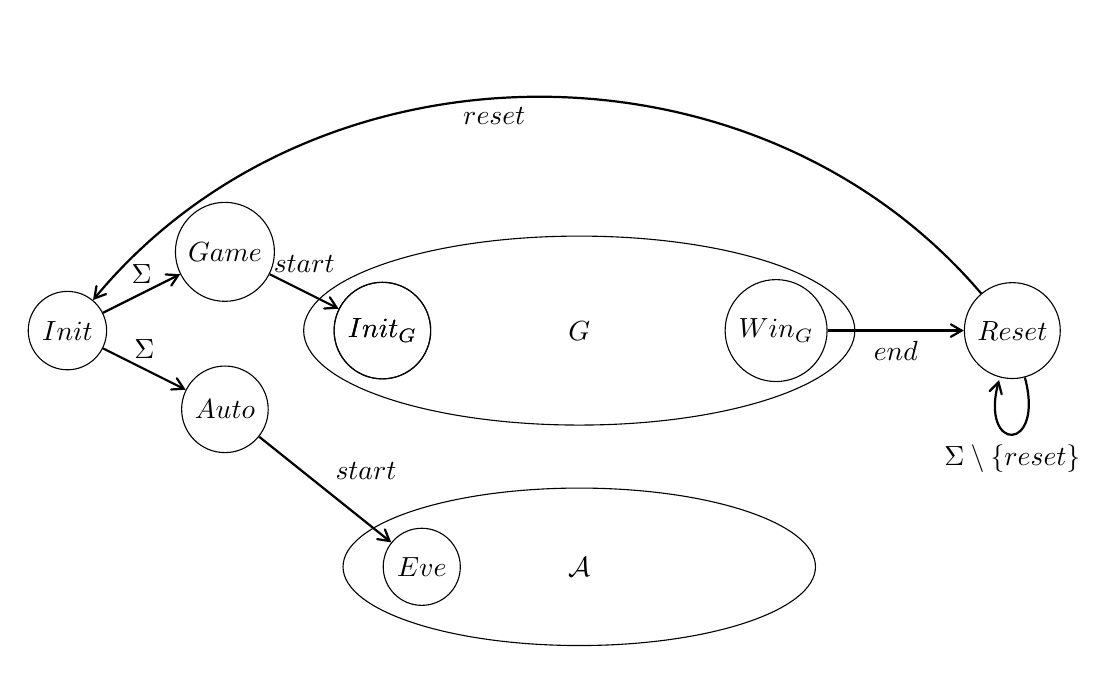
\begin{tikzpicture}
		\node[state] (A) at (-2,0) {$Init$};
		\node[state] (C) at (2, 0) {$Init_G$};
		\node[state] (B) at (10,0) {$Reset$};
		\node[state] (C) at (2, 0) {$Init_G$};
		\node[state] (D) at (7, 0) {$Win_G$};
		\node[state] (H) at (0,1) {$Game$};
		\node[state] (I) at (0,-1) {$Auto$};
		\node (J) at (4.5,0) {$G$};
		\node (J) at (4.5,-3) {$\mathcal{A}$};
		\node[state] (K) at (2.5,-3) {$Eve$};
		
		\draw (4.5,0) ellipse (3.5 and 1.2);
		\draw (4.5,-3) ellipse (3 and 1);
		
		\path[->, thick, >=angle 60] (H) edge node[above=3pt] {$start$} (C);
		\path[->, thick, >=angle 60] (I) edge node[above right] {$start$} (K);
		\path[->, thick, >=angle 60] (A) edge node[above] {$\Sigma$} (H);
		\path[->, thick, >=angle 60] (A) edge node[above] {$\Sigma$} (I);
		\path[->, thick, >=angle 60] (D) edge node[below] {$end$} (B);
		\path[->, thick, >=angle 60, bend right=50] (B) edge node[below left] {$reset$} (A);
		\path[->, thick, >=angle 60, loop below] (B) edge node[below] {$\Sigma\setminus\set{reset}$} (B);
	\end{tikzpicture}
	\caption{Transition system for the non-stochastic reduction}
	\label{fig-nsreach1}
\end{figure}

\begin{figure}[h]
	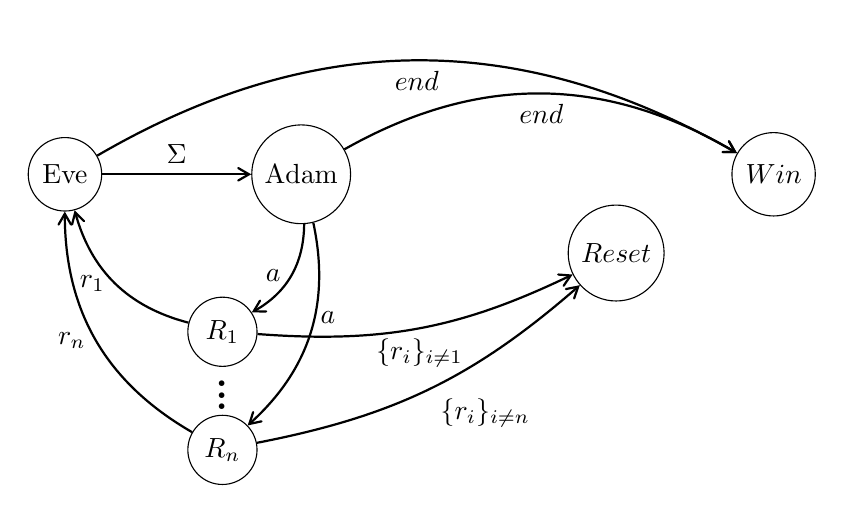
\begin{tikzpicture}
	\node[state] (A) at (0,0) {Eve};
	\node[state] (B) at (3,0) {Adam};
	\node[state] (C) at (2, -2) {$R_1$};
	\node[state] (D) at (2, -3.5) {$R_n$};
	\node (E) at (2,-2.7) {\Huge \vdots};
	\node[state] (F) at (7,-1) {$Reset$};
	\node[state] (G) at (9,0) {$Win$};
	
	
	\path[->, thick, >=angle 60] (A) edge node[above] {$\Sigma$} (B);
	\path[->, thick, >=angle 60, bend left = 30] (B) edge node[left] {$a$} (C);
	\path[->, thick, >=angle 60, bend left = 30] (B) edge node[above right] {$a$} (D);
	\path[->, thick, >=angle 60, bend left = 30] (C) edge node[left] {$r_1$} (A);
	\path[->, thick, >=angle 60, bend left = 30] (D) edge node[left] {$r_n$} (A);
	\path[->, thick, >=angle 60, bend right = 15] (C) edge node[below] {$\set{r_i}_{i \neq 1}$} (F);
	\path[->, thick, >=angle 60, bend right = 15] (D) edge node[below right] {$\set{r_i}_{i \neq n}$} (F);
	\path[->, thick, >=angle 60, bend left = 30] (A) edge node[below] {$end$} (G);
	\path[->, thick, >=angle 60, bend left = 30] (B) edge node[below] {$end$} (G);
	
	\end{tikzpicture}
	\caption{Transition system $\mathcal{A}$ from Figure \ref{fig-nsreach1}}
	\label{fig-nsreach2}
\end{figure}


\section{Stochastic reachability}

We show that the problem of deciding the winner of a two-player stochastic population game is undecidable by reduction from the reachability problem for a two-counter Minsky machine.

Let $\mathcal{M} = (Q, \Delta, init, fin)$ be such a machine, a configuration being an element of $Q \times \nats^2$, with $\Delta \subseteq Q \times \set{++, --, =0?} \times \set{1,2} \times Q$ with the usual semantics.

We describe our construction in several steps: We start with a general map of the system, drawn in Figure~\ref{fig-sreach1}.

\begin{figure}[h]
	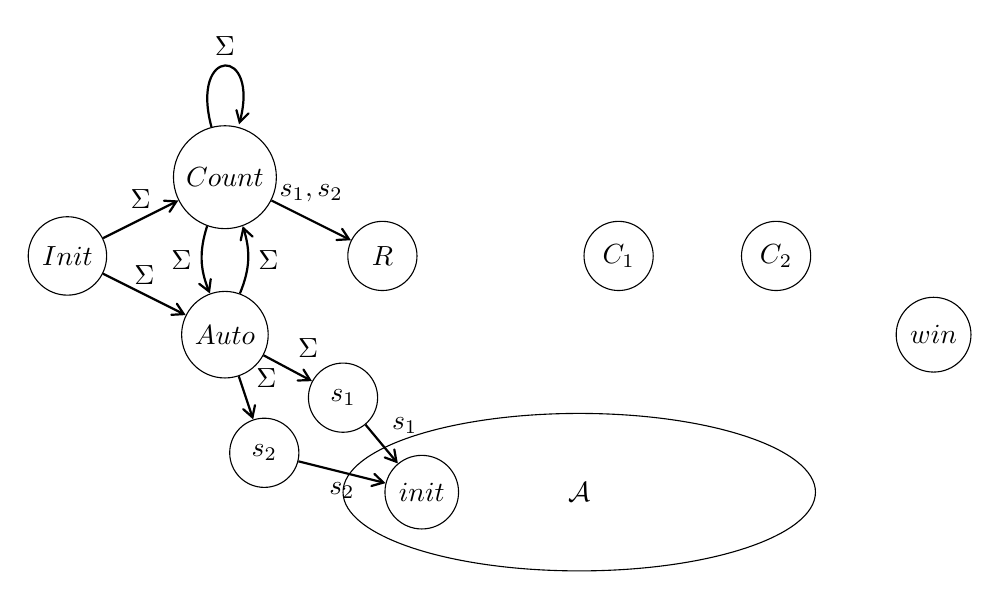
\begin{tikzpicture}
		\node[state] (A) at (-2,0) {$Init$};
		\node[state] (C) at (2, 0) {$R$};
		\node[state] (E) at (5, 0) {$C_1$};
		\node[state] (D) at (7, 0) {$C_2$};
		\node[state] (D) at (9, -1) {$win$};
		\node[state] (H) at (0,1) {$Count$};
		\node[state] (I) at (0,-1) {$Auto$};
		\node (J) at (4.5,-3) {$\mathcal{A}$};
		\node[state] (S1) at (1.5,-1.8) {$s_1$};
		\node[state] (S2) at (0.5,-2.5) {$s_2$};
		\node[state] (K) at (2.5,-3) {$init$};
		
		\draw (4.5,-3) ellipse (3 and 1);
		
		\path[->, thick, >=angle 60, bend right=20] (H) edge node[left] {$\Sigma$} (I);
		\path[->, thick, >=angle 60, bend right=20] (I) edge node[right] {$\Sigma$} (H);
		\path[->, thick, >=angle 60, loop above] (H) edge node[above] {$\Sigma$} (H);
		\path[->, thick, >=angle 60] (H) edge node[above=3pt] {$s_{1}, s_2$} (C);
		\path[->, thick, >=angle 60] (I) edge node[above right] {$\Sigma$} (S1);
		\path[->, thick, >=angle 60] (I) edge node[above right] {$\Sigma$} (S2);
		\path[->, thick, >=angle 60] (S1) edge node[above right] {$s_1$} (K);
		\path[->, thick, >=angle 60] (S2) edge node[below] {$s_2$} (K);
		\path[->, thick, >=angle 60] (A) edge node[above] {$\Sigma$} (H);
		\path[->, thick, >=angle 60] (A) edge node[above] {$\Sigma$} (I);
		\end{tikzpicture}
		\caption{Transition system for the stochastic reduction. There are transitions $reset$ from $s_1$ and $s_2$ to $win$, and from $Count$ and $Auto$ to $Init$}
	\label{fig-sreach1}
\end{figure}

At the start Eve chooses how to spread tokens between the places $Count$ and $Auto$. 
However she does not have a real choice: putting more than one token in $Auto$ will give her a positive probability to lose (if tokens go to $s_1$ and $s_2$) while putting no tokens in $Auto$ will allow Adam to reset the game for free.

However if Adam tries to reset the game while Eve did put tokens in Auto, those are sent to the winning state and the game restarts with less tokens, disadvantaging Adam. 

As a result, the players' best choices lead to a configuration where all tokens are in $Count$ except for one which is in $Auto$. We can then start the simulation of $\mathcal{M}$.

The simulation will proceed by rounds, with each round going as follows:
\begin{itemize}
	\item Adam chooses a transition (and commits to that transition being feasible).
	
	\item Eve executes the associated operation on the counters, and has the opportunity to punish Adam if the chosen transition is not possible.  
\end{itemize}

If the reserve gets empty then Adam loses. If state $fin$ is reached then Adam wins as it is a sink state. Both players may reset the game to punish each other for cheating. The difference is that Eve will punish Adam by resetting the game while sending some tokens to the winning state, while Adam will punish Eve by sending all tokens (outside the winning state) to the start.

If at any point the reserve $R$ is empty, Eve has an action to send all tokens to $win$ (which also sends tokens of $R$ to $fin$ if it is not empty).

Concretely, there is a place in $\mathcal{A}$ for each state in $Q$ and one for each transition $t \in \Delta$.

From each state Adam will choose an outgoing transition, and the token will stay on the associated place while the operation is checked and executed, after which it will be transferred to the target state of said transition.

For a zero test $=0?$ on counter $C_i$, Eve is allowed to send all tokens (except those of $win$ and $fin$) to the $Start$ state, except those of $C_i$ which are sent to $win$, and those of places of $\mathcal{A}$ not of the form $(q_1, =0?, i, q_2)$ to $fin$.

Hence Eve can only apply that action when Adam chose a transition that tests the emptiness of $C_i$. If $C_i$ was not empty the game restarts with less tokens, advantaging Eve. 
If $C_i$ was indeed empty, then Eve made no progress.

Thus the best move for Eve is to reset the game that way iff Adam chose a transition of the form $(q_1, =0?, i, q_2)$ and $C_i$ is not empty. 

For an increment $++$ (resp. decrement) on counter $C_i$, Eve chooses a number of tokens to transfer from $R$ to $C_i$ (resp. from $C_i$ to $R$). The mechanism is the same as the one at the start when she chose the number of tokens to send to $Auto$.

If she chooses more than one token she has a positive probability that the tokens split and go to different states, causing her to lose. If she chooses zero, then Adam can reset the game for free (at the condition that the token in $\mathcal{A}$ is indeed in a place of the form $(q_1, ++, i, q_2)$).

If $R$ is empty and the token in $\mathcal{A}$ is in a place of the form $(q_1, ++, i, q_2)$ she can send all tokens to win and win.

Hence Adam has a winning strategy if and only if $fin$ is reachable in $\mathcal{M}$.

\newpage

\section{Safety}

This is much simpler: Say we ignore the tokens and simply play a safety game on the graph. At each state the player who owns it chooses a letter and Adam chooses one of the states accessible by a transition with that letter. If Eve wins then she has an attractor containing the initial state and within the safe area, meaning that she can keep all tokens within that zone and thus win. 

If Adam wins he does so in at most $n$ steps ($n$ being the number of states). In order to win the game with tokens he simply has to put $d^n$ (with $d$ the degree of the graph) tokens in the initial state, allowing him to simulate his strategy in the safety game until he wins without running out of tokens. This holds whether tokens behave in a stochastic or adversarial way, as Eve has to guarantee a winning probability of one.

\section{Undecidability of verification of $\set{0,1, \omega}$ strategies}

Consider a two-counter system $\S = (S, \delta, init, fin)$ with $\delta : S \times \set{\top, \bot}^2 \to \set{1,2} \times Op \times S$ and $Op = \set{++, --}$.
Intuitively, $\delta$ takes as input the current state and two booleans indicating if the counters are equal to $0$ or not. It outputs an operation, a counter on which to apply it and a new state.

Note that this machine has a single run from its initial configuration $(init, 0, 0)$.
The problem whether such a machine is unbounded (that is, one of its counters reaches arbitrarily high values along its run) is undecidable.

Consider the following population game: There is a place for each state $s \in S$, two places for each counter, two more forming a reservoir of tokens, plus a starting and a final place.

We have an action for each $(s, b1, b2) \in S \times \set{\top, \bot}^2$, plus special letters $start, empty, win, shuffle$.

The letter $start$ takes all tokens from the starting place and splits them between the reservoir and the place associated to $init$.
The letter $empty$ can only be played if all places associated with states are empty, and it sends all tokens to the final place.
As for $win$, it can only be played if the reservoir is empty, and it sends all tokens to the final place.
Finally, $shuffle$ redistributes randomly the tokens between each pair of states associated with the reservoir and each counter.

For each $(s, b1, b2)$, with $\delta(s, b1, b2) = (i, op, t)$, the associated action can only be played if all places associated with states besides $s$ are empty, and transfers the ones in $s$ to $t$.

If $op = ++$ then it transfers all tokens from one of the two places of the reservoir to counter $i$.
If $op = --$ then it transfers all tokens from one of the two places of counter $i$ to the reservoir.

We consider the strategy that consists in executing faithfully the two-counter machine. It starts by executing $start$. If no token reaches the places associated with states, it reads $empty$ and wins.

Otherwise it executes $shuffle$ until in the three pairs of places associated with the counters and the reservoir the tokens are split between one token on a side and all others on the other side.

Then it reads the action associated with $s, b1, b2$, where $s$ is the unique state where there are tokens, and $b1$ and $b2$ are true if, respectively, there are no tokens in the states of counters $1$ and $2$. Thanks to the previous paragraph, we know that exactly one token is transferred from the decremented counter to the reservoir, or from the reservoir to the incremented counter.

If at any point the reservoir is empty, it plays action $win$.

An easy induction shows that if the play yielded by this strategy goes through $n$ actions $(s,b1, b2)$, then those are the $n$ first actions of the machine, and if the configuration of the machine after executing them is $(s, c1, c2)$, then the the resulting configuration in the game is such that 
\begin{itemize}
	\item There are tokens in $s$ but not in any other state $t$.
	
	\item There are $c1$ tokens in total in the two places of counter $1$, and $c2$ in the places of counter $2$.
\end{itemize}

As a result if the machine is bounded by a bound $B$, then if at the start there are $2B + 2$ tokens, there is a positive probability that one of them is sent to the states, and $2B+1$ to the reservoir at the start. Then the reservoir will never be empty (as there are at most $2B$ tokens in the counters and one in the states and zero elsewhere at all times), and neither will the states. Hence the strategy is not winning.

If the machine is unbounded, then let $N \in \nats$, say we start with $N$ tokens.
If none of them are sent to the states then we win immediately by playing $empty$.
Otherwise there are $K < N$ tokens sent to the reservoir. The strategy simulates the machine until we reach a configuration where the sum of the counters is above $K$ (which happens eventually as it is unbounded). Then we play $win$ and win.

As a result, the strategy is winning if and only if the machine is unbounded.
Furthermore this strategy bases its decisions solely on the $0, 1, \omega$ abstraction of the current configuration.

As a consequence, the verification of a (positional) $(0, 1, \omega)$ strategy for population games is undecidable.

\section{Very weak automata}

We consider automata equipped with a total order $\leq$ on their states such that all transitions $(s, a, t)$ are such that $s \leq t$. We aim at determining the complexity of solving population games over such automata.

\subsection{Lower bound}

Here is a PSPACE lower bound: 

We reduce the emptiness problem for Zielonka automata. Those are automata over a set $Proc$ of processes, with a family of sets of states $(S_p)_{p \in Proc}$, another of initial states $(init_p)_{p \in Proc}$, a set of global final states $F \subseteq \Pi_{p\in Proc} S_p$ and transitions of the form $(s_{p_1}, \ldots, s_{p_k}) \xrightarrow{a} (s'_{p_1}, \ldots, s'_{p_k})$, with $p_1, \ldots, p_k \in Proc$.

We set up the following game: 

It consists of two parts: One will be in charge of simulating the effect of the sequence of actions chosen by the player on the configuration of the automaton.

The other is a timer (in the form of a binary counter) ensuring that at most  $M = \Pi_{p\in Proc} |S_p|$ are played.

We first describe the automaton simulation: 

We have a reservoir of tokens, and one place for each state of each process.
The actions are the transitions of the automaton. The effect of an action $(s_{p_1}, \ldots, s_{p_k}) \xrightarrow{a} (s'_{p_1}, \ldots, s'_{p_k})$ is to send all tokens from the $s_{p_i}$ to the target place, kill all tokens in the other states of the $p_i$, split the tokens of the reservoir between itself and the $s'_{p_i}$ and loop on all states of all other processes.

For all $(f_p)_{p \in Proc} \in F$ we have an action that sends all tokens from the $f_p$ and the reservoir to the target place, and kills all other places. 

Observe that if the automaton accepts a word, then it accepts one of size less than $M$, and we can send all tokens to the target place by reading an accepting sequence of that word, then the action corresponding to the final configuration reached.  

Now suppose we can send all tokens to the target with $M$ actions, then by starting with a large enough number of tokens, there is a positive probability that all splits of the reservoir send at least one token in all its successors. As a result, a winning run in $M$ moves has to simulate a run of the automaton. 
In order to be winning, it needs to end with some $f \in F$, hence the corresponding run is accepting. 

Now we describe the other part of the game, playing in parallel.
We set $n$ as the integer part of $log_2(M)+1$. We have $2n$ places, of the form $(j,b)$ with $0 \leq j \leq  n$ and $b \in \set{0,1}$, plus a reservoir.
An action is a number $0\leq i < n$. Its effect is to send all tokens of $(i', 0)$ to $(i', 1)$ and kill those in $(i',1)$ for all $i'\leq i$. It also kills the tokens in $(i,0)$, sends the tokens of $(i,1)$ to the target and splits the tokens of the reservoir between itself and $(i,0)$. It leaves the rest untouched.

For each $i$ there is also an action $end_i$ which kills all tokens in $(i,0)$ and sends all others to the target state.

Now we describe the entire game: We take the union of the two parts described above, plus initial and final places. At first the tokens of the initial place are split between the reservoirs of the two parts, as well as the places $(init_p)_{p \in Proc}$ and $(i,1)$.

Then the rest of the actions are pairs $(x,y)$ with $x$ an action of the automaton part and $y$ an action of the counter part.

Their effects are applied independently on each part of the graph.

Suppose there is an accepting run of the automaton, then there is one of length less than $M < 2^n$, hence we can play the corresponding actions in the automaton part while decreasing the counter in the other part at each step.
In the end the counter has not reached $0$, hence there is an $i$ such that $(i,0)$ is empty. Meanwhile, the automaton has reached a final configuration $f \in F$, hence we can play $(end_i, f)$ and win.

Now suppose there is a winning strategy. We can assume that are numerous enough so that during the first $M$ steps of the play every reached enabled transition is taken by some tokens at all times.

As a consequence, such a play cannot last more than $M$ steps, as otherwise the binary counter would reach $0$, with tokens in all $(i,0)$ places, meaning that no action can be played without killing some of them.
Hence in the automaton part we had to follow an accepting run.

\subsection{Upper bound}


  
\printbibliography

\end{document}